\documentclass[12pt,letterpaper, onecolumn]{exam}
\usepackage{amsmath}
\usepackage{amssymb}
\usepackage{sidecap}
\usepackage{tabularx}
\usepackage{csquotes}
\usepackage{makecell}
\usepackage{hyperref}
\hypersetup{
    colorlinks=true,
    linkcolor=blue,
    filecolor=magenta,      
    urlcolor=black,
    pdftitle={Overleaf Example},
    pdfpagemode=FullScreen,
}
%\usepackage[left=0.5cm,right=0.5cm,top=0.5cm,bottom=0.5cm]{geometry}
\usepackage[usestackEOL]{stackengine}
%\setstacktabbedgap{1ex} 
\usepackage{tikz}
\usetikzlibrary{decorations.pathreplacing}
\usetikzlibrary{fadings}
\def\layersep{2.5cm}

\usepackage{enumitem}
\usepackage{graphicx}
\usepackage{algorithm}
\usepackage{algpseudocode}

\usepackage{subcaption}

%\usepackage[shortlabels]{enumitem}
%\usepackage{enumerate}
\usepackage[lmargin=71pt, tmargin=0.8in]{geometry}  %For centering solution box

% \chead{\hline} % Un-comment to draw line below header
\thispagestyle{empty} 
  %For removing header/footer from page 1
\usepackage{color}
\definecolor{light-gray}{gray}{0.95}

\usepackage{listings}
\lstset{
    basicstyle=\footnotesize\ttfamily,
    escapechar=¢,
    language=python,
    frame=single,
    frameround=tttt,
    showstringspaces=false,
    backgroundcolor=\color{light-gray}
}  %For removing header/footer from page 1


\usepackage{xcolor}

\definecolor{codegreen}{rgb}{0,0.6,0}
\definecolor{codegray}{rgb}{0.5,0.5,0.5}
\definecolor{codepurple}{rgb}{0.58,0,0.82}
\definecolor{backcolour}{rgb}{0.95,0.95,0.92}

\lstdefinestyle{mystyle}{
    backgroundcolor=\color{light-gray},   
    commentstyle=\color{codegreen},
    keywordstyle=\color{magenta},
    numberstyle=\tiny\color{codegray},
    stringstyle=\color{codepurple},
    basicstyle=\ttfamily\footnotesize,
    breakatwhitespace=false,         
    breaklines=true,                 
    captionpos=b,                    
    keepspaces=true,                 
    numbers=left,                    
    numbersep=5pt,                  
    showspaces=false,                
    showstringspaces=false,
    showtabs=false,                  
    tabsize=2
}

\lstset{style=mystyle}




\begin{document}



\newtheorem{theorem}{Theorem}[section]
\newtheorem{problem}{Problem}
\newtheorem{proposition}{Proposition}[section]
\newtheorem{lemma}{Lemma}[section]
\newtheorem{corollary}[theorem]{Corollary}
\newtheorem{example}{Example}[section]
\newtheorem{definition}[problem]{Definition}

\newcommand{\BEQA}{\begin{eqnarray}}
\newcommand{\EEQA}{\end{eqnarray}}
\newcommand{\define}{\stackrel{\triangle}{=}}
\bibliographystyle{IEEEtran}
\raggedbottom
\setlength{\parindent}{0pt}
\providecommand{\mbf}{\mathbf}
\providecommand{\norm}[1]{\lVert#1\rVert}
\providecommand{\pr}[1]{\ensuremath{\Pr\left(#1\right)}}
\providecommand{\qfunc}[1]{\ensuremath{Q\left(#1\right)}}
\providecommand{\sbrak}[1]{\ensuremath{{}\left[#1\right]}}
\providecommand{\lsbrak}[1]{\ensuremath{{}\left[#1\right.}}
\providecommand{\rsbrak}[1]{\ensuremath{{}\left.#1\right]}}
\providecommand{\brak}[1]{\ensuremath{\left(#1\right)}}
\providecommand{\lbrak}[1]{\ensuremath{\left(#1\right.}}
\providecommand{\rbrak}[1]{\ensuremath{\left.#1\right)}}
\providecommand{\cbrak}[1]{\ensuremath{\left\{#1\right\}}}
\providecommand{\lcbrak}[1]{\ensuremath{\left\{#1\right.}}
\providecommand{\rcbrak}[1]{\ensuremath{\left.#1\right\}}}
\let\vec\mathbf

\newlist{mydesc}{description}{1} % create a new list called mydesc, of type "description"
\setlist[mydesc]{
  align=left, % use the align-format defined above
  leftmargin=0pt, % indentation for all the lines
  labelindent=1em, % horizontal space before label
  labelsep=0pt
   % horizontal space after label -- set to zero because we add space via "leftwithbar"
}



\begingroup  
    \centering
    
    \LARGE Weekly Report 3 - XGBoost\\[0.5em]
    
    \large Ganji Varshitha\par
    \large AI20BTECH11009\par
\endgroup
\rule{\textwidth}{0.4pt}
\pointsdroppedatright   %Self-explanatory
\printanswers
\newcommand\Solution{
  \textbf{Solution:}\\}
\newcommand{\myvec}[1]{\ensuremath{\begin{bmatrix}#1\end{bmatrix}}}
 %Replace "Ans:" with starting keyword in solution box

\subsection*{Introduction}
XGBoost stands for Extreme Gradient Boosting algorithm. It is an enhanced GBM model. It improves the performance and speed of model.
It provides parallel tree boosting and works very fast than GBMs.\\
It is a supervised learning ensemble model.
\subsection*{Algorithm}
The GBM algorithm is modified with few regularization factors in XGBoost algorithm.\\
\begin{figure}[!h]
\centering
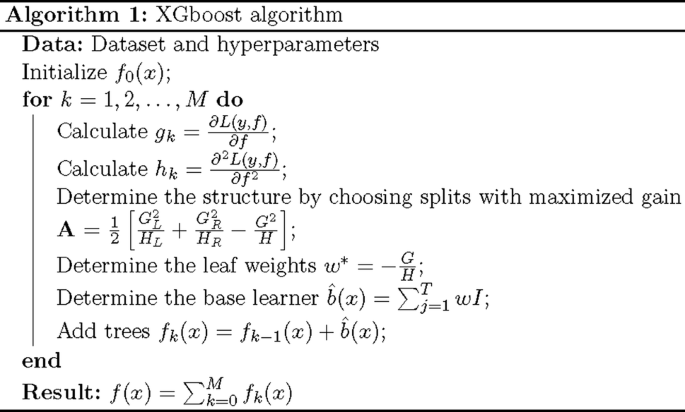
\includegraphics[width = \textwidth]{../images/xgboost}
\end{figure}

\subsection*{Optimizations}
\subsubsection*{ System optimizations}
\begin{itemize}
\item Parallelization: XGboost can take use of multiple cores of CPU. Data stores in memory units called blocks which can be reused in the algorithm.

\item Distributed Computing for training very large models using a cluster of machines.
\item Out-of-Core Computing for very large datasets that don’t fit into memory.
\item Hardware Optimisation: Cache Optimization of data structures and algorithm to make best use of hardware.
\end{itemize}

\subsubsection*{Algorithm features}
\begin{itemize}
\item Regularization: It uses LASSO(L1) and ridge(L2) regularization. This prevents overfitting.
\item Cross validation: The algorithm has inbuilt cross validation at every iteration of training.
\item Tree pruning: It follows depth first search approach. The algorithm prunes the tree in backward direction.
\end{itemize}






\subsection*{Questions}



\end{document}